\documentclass{article}
\usepackage{amsfonts, amsmath, amssymb, amsthm, dsfont} % Math notations imported
\usepackage{enumitem}
\usepackage{graphicx}
\usepackage{setspace}
\usepackage{indentfirst}
\usepackage[margin=1in]{geometry}
\graphicspath{{./images/}} % Path to images

% \begin{figure}[htb!]
%      \centering
%      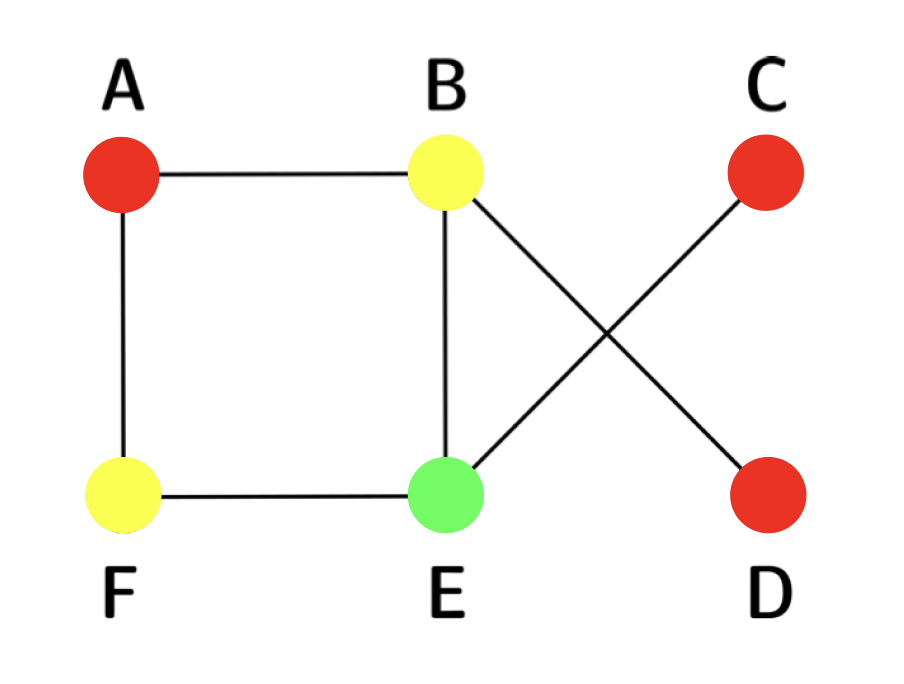
\includegraphics[scale=0.5]{coloring.png}
%      \caption{Coloring of the graph.}
% \end{figure}

% \begin{figure}[htb]
%     \qquad
%     \begin{minipage}{.4\textwidth}
%         \centering
%         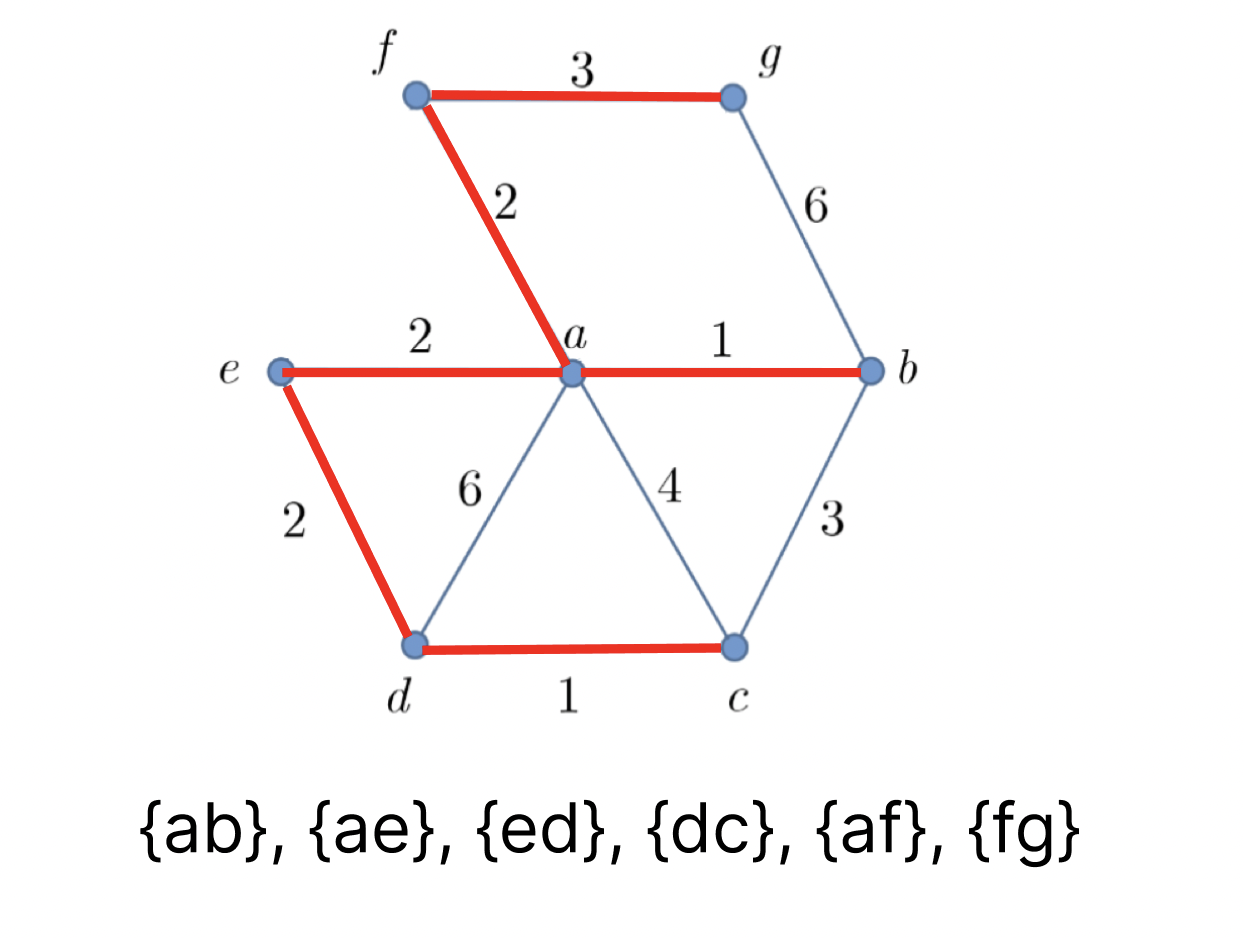
\includegraphics[scale=0.35]{prims.png}
%         \caption{}
%     \end{minipage}    
%     \qquad
%     \begin{minipage}{.4\textwidth}
%         \centering
%         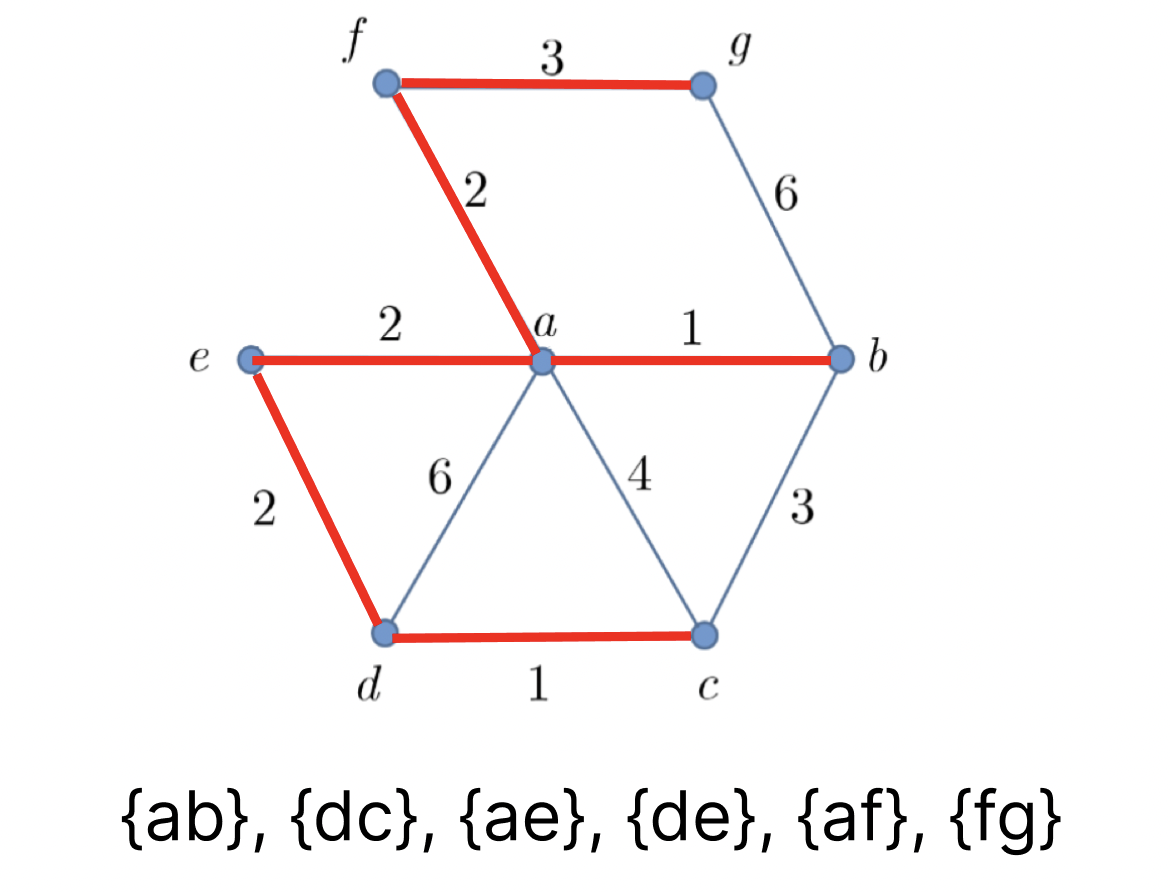
\includegraphics[scale=0.35]{kruskal.png}
%         \caption{}
%     \end{minipage}        
% \end{figure} 

\newtheorem{thm}{Theorem}
\newtheorem{proposition}[thm]{Proposition}
\newtheorem{corollary}[thm]{Corollary}
\newtheorem{lemma}[thm]{Lemma}

\newcommand*{\Var}{\ensuremath{\mathrm{Var}}}
\newcommand*{\Cov}{\ensuremath{\mathrm{Cov}}}
\newcommand*{\Corr}{\ensuremath{\mathrm{Corr}}}
\newcommand*{\Bias}{\ensuremath{\mathrm{Bias}}}
\newcommand*{\MSE}{\ensuremath{\mathrm{MSE}}}
\newcommand*{\range}{\ensuremath{\mathrm{range}}\,}
\newcommand*{\spann}{\ensuremath{\mathrm{span}}\,}
\newcommand*{\nul}{\ensuremath{\mathrm{null}}\,}
\newcommand*{\dom}{\ensuremath{\mathrm{dom}}\,}
\renewcommand*{\implies}{\ensuremath{\Longrightarrow}}
\renewcommand*{\impliedby}{\ensuremath{\Longleftarrow}}
\newcommand*{\Z}{\ensuremath{\mathbb{Z}}}
\newcommand*{\Q}{\ensuremath{\mathbb{Q}}}
\newcommand*{\R}{\ensuremath{\mathbb{R}}}
\newcommand*{\F}{\ensuremath{\mathbb{F}}}
\newcommand*{\C}{\ensuremath{\mathbb{C}}}
\newcommand*{\N}{\ensuremath{\mathbb{N}}}
\newcommand*{\E}{\ensuremath{\mathds{E}}}
\renewcommand*{\P}{\ensuremath{\mathds{P}}}
\newcommand*{\p}{\ensuremath{\mathcal{P}}}

% title information
\title{Math 104 HW8}
\author{Neo Lee}
\date{11/03/2023}

\setstretch{1.15}
% main content
\begin{document} 

% placing title information; comment out if using fancyhdr
\maketitle 


\subsection*{Exercise 19.1}
Which of the following continuous functions are uniformly continuous on the specified set? \\
\textbf{(b)} $f(x)=x^3$ on [0, 1] \qquad \textbf{(d)} $f(x)=x^3$ on \R \qquad \textbf{(f)} $f(x)=\sin\frac{1}{x^2}$ on (0,1] 
\qquad \textbf{(g)} $f(x)=x^2\sin\frac{1}{x}$ on (0,1].
\begin{proof}[Solution]\indent
    \begin{enumerate}
        \item [\textbf{(b)}] $f(x)=x^3$ is continous on \R, and hence continuous on 
        [0, 1]. By \emph{Theorem 19.2}, $f$ is uniformly continuous on [0,1].

        \item [\textbf{(d)}] $f(x)=x^3$ is not uniformly continuous on \R. Assume for the sake of 
        contradiction that for any $\epsilon>0$ there exists $\delta>0$ such that for all $x,y\in\R$, $|x-y|<\delta \implies 
        |f(x)-f(y)|=|x^3-y^3|<\epsilon$. However, consider $y>0$ and 
        $x=y+\frac{\delta}{2}$, then $|x^3-y^3|=x^3-y^3=(x-y)(x^2+xy+y^2)=\frac{\delta}{2}\left((y+\frac{\delta}{2})^2
        +(y+\frac{\delta}{2})y+y^2\right)$, which is unbounded as $y\to\infty$. Hence, there exists 
        $y>0$ and $x=y+\frac{\delta}{2}$ such that $|x-y|<\delta \not\implies 
        |f(x)-f(y)|=|x^3-y^3|<\epsilon$.

        \item [\textbf{(f)}] Let a sequence $(s_n)=\frac{1}{n}$, which is obviously convergent and 
        hence Cauchy on (0, 1]. However, notice $(f(s_n))=\sin n^2$ is not convergent [there are 
        always $n>N$ such that $\sin n^2$ is not within the $\epsilon$ neighborhood of any potential 
        limit]. Hence, $(f(s_n))$ is not Cauchy, and by \emph{Theorem 19.4}, $f$ is not 
        uniformly continuous.

        \item [\textbf{(g)}] Extend $f$ to $\tilde{f}$ by defining $\tilde{f}(0)=0$, 
        then $\tilde{f}$ is continuous at 0 because for $x\neq0$ and $|x-0|<\sqrt{\epsilon}$, 
        $|x^2\sin\frac{1}{x}-0|\le |x^2| < \epsilon$. Hence, $\tilde{f}$ is continuous on 
        [0, 1] and by \emph{Theorem  19.5}, $f$ is uniformly continuous on $(0,1)$. Then 
        also notice $f$ is continuous on the interval $[0.5,1]$, hence is uniformly continuous on 
        $[0.5,1]$ by \emph{Theorem 19.2}. Then take $\delta=\min\{\delta_1, \delta_2, 0.5\}$, 
        where $\delta_1$ and $\delta_2$ represent the guaranteed $\delta$ for $f$ on $(0,1)$ and 
        $[0.5,1]$ respectively. Since $\delta\le 0.5$, $x,y$ must both in $[0.5,1]$ or $(0,1)$, and 
        $|x-y|<\delta \implies |f(x)-f(y)|<\epsilon$ for $x,y\in(0,1]$.
    \end{enumerate}
    
\end{proof}

\subsection*{Exercise 19.4}
\begin{enumerate}
    \item [\textbf{(a)}] 
    \begin{proposition}
        If f is uniformly continuous on a bounded set S, then f is a bounded function on 
        S.
    \end{proposition}
    \begin{proof}
        Assume for the sake of contradiction that $f$ is unbounded on $S$. We will consider the 
        case for unbounded above here, and the case for unbounded below is analogous, which will be 
        omitted. Since 
        $f$ is unbounded above on $S$, for any $n\in\N$, there exists $x_n\in S$ such that
        $f(x_n)>n$. Since $S$ is bounded, $(x_n)$ is bounded, and hence by Bolzano-Weierstrass
        theorem, there exists a convergent subsequence $(x_{n_k})$ of $(x_n)$.

        Now consider this subsequence $(x_{n_k})$, which is Cauchy since it is convergent. 
        We already know $f$ is uniformly continuous on $S$, hence by \emph{Theorem 19.4}, $(f(x_{n_k}))$
        is a Cauchy sequence, hence convergent. However, since $f(x_{n_k})>n_k$, $(f(x_{n_k}))$
        is not convergent, which is a contradiction. Hence, $f$ must be bounded on $S$.
    \end{proof}

    \newpage
    \item [\textbf{(b)}] Use \textbf{(a)} to give a proof that $\frac{1}{x^2}$ is not uniformly 
    continuous on (0, 1).
    \begin{proof}
        Consider $f=\frac{1}{x^2}$ on (0, 1), which is a bounded set. However, $f$ is unbounded 
        above on $(0, 1)$ because consider the sequence $(x_n)=\frac{1}{n}$, 
        $\lim f(x_n)=\lim n^2=\infty$, which means there always $\exists x_n\in (0,1)$
        such that $f(x_n)>M\in\R^+$. Hence, by \textbf{(a)}, $f$ is not uniformly continuous on
        $(0,1)$.
    \end{proof}
\end{enumerate}

\subsection*{Exercise 20.6}
\begin{proposition}
    Let f = $\frac{x^3}{|x|}$, then $\lim_{x\to\infty}f(x)=\infty, \lim_{x\to-\infty}f(x)=-\infty, 
    \lim_{x\to0}f(x)=\lim_{x\to0^+}f(x)=\lim_{x\to0^-}f(x)=0$.
\end{proposition}
\begin{proof}
    Notice $$f=\begin{cases}
        x^2 & x>0 \\
        -x^2 & x<0.
    \end{cases}$$

    To prove $\lim_{x\to\infty}f(x)=\infty$, consider the interval $(1,\infty)$. Then for any 
    sequence $(x_n)\in (1,\infty)$ with $\lim x_n=\infty$, we have $\lim f(x_n)=\infty$ because
    for each $M>0$, there exists $N\in\N$ such that $x_n>M$ for all $n>N$ \implies 
    $f(x_n)=x_n^2\ge x_n > M$ for all $n>\N$.

    Similarly, to prove $\lim_{x\to-\infty}f(x)=-\infty$, consider the interval $(-\infty,-1)$. 
    Then for any sequence $(x_n)\in (-\infty,-1)$ with $\lim x_n=-\infty$, we have
    $\lim f(x_n)=-\infty$ because for each $M<0$, there exists $N\in\N$ such that
    $x_n<M$ for all $n>N$ \implies $f(x_n)=-x_n^2\le x_n < M$ for all $n>\N$.

    To prove $\lim_{x\to0^+}f(x)=0$, consider the interval $(0,1)$, then for any sequence 
    $(x_n)\in (0,1)$ with $\lim x_n=0$, we have $\lim f(x_n)=\lim x_n\cdot x_n=0\cdot 0=0$.

    Similarly, to prove $\lim_{x\to0^-}f(x)=0$, consider the interval $(-1,0)$, then for any
    sequence $(x_n)\in (-1,0)$ with $\lim x_n=0$, we have $\lim f(x_n)=\lim x_n\cdot x_n=0\cdot 0=0$.

    Finally, by \emph{Theorem 20.10}, since $\lim_{x\to0^+}f(x)=\lim_{x\to0^-}f(x)=0$, 
    $\lim_{x\to0}f(x)=0$.
\end{proof}

\subsection*{Exercise 20.16}
\begin{proposition}
    Suppose that limits $L_1=\lim_{x\to a^+}f_1(x)$ and $L_2=\lim_{x\to a^+}f_2(x)$ 
    exists. 
    \begin{enumerate}
        \item [\textbf{(a)}] If $f_1(x)\le f_2(x)$ for all $x$ in some intervale $(a,b)$, 
        then $L_1\le L_2$.

        \item [\textbf{(b)}] If $f_1(x)<f_2(x)$ for all x in some interval $(a,b)$, 
        $L_1$ is not necessarily less than $L_2$.
    \end{enumerate}
\end{proposition}
\begin{proof}
    \begin{enumerate}
        \item [\textbf{(a)}] Assume for the sake of contradiction that $L_1 > L_2$. Then, 
        there exists some sequence $(x_n)\in(a,b)$ with $\lim x_n=a$ such that $\lim f_1(x_n)=L_1$ 
        while $\lim f_2(x)=L_2<L_1$.

        Now denote $\epsilon = L_1-L_2$, then there exists $N_1\in\N$ such that for all $n>N_1$, 
        $|f_1(x_n)-L_1|<\frac{\epsilon}{2}\implies f_1(x_n)\in(L_1-\frac{\epsilon}{2},L_1+\frac{\epsilon}{2})$. Also, 
        there exists $N_2\in\N$ such that for all $n>N_2$,
        $|f_2(x_n)-L_2|<\frac{\epsilon}{2}\implies f_2(x_n)\in(L_2-\frac{\epsilon}{2},L_2+\frac{\epsilon}{2})$. 
        Then, for all $n>\max\{N_1,N_2\}$, $f_1(x_n)\in(L_1-\frac{\epsilon}{2},L_1+\frac{\epsilon}{2})$ and
        $f_2(x_n)\in(L_2-\frac{\epsilon}{2},L_2+\frac{\epsilon}{2})$, which means $f_1(x_n)>f_2(x_n)$, which is a
        contradiction. Hence, $L_1\le L_2$.

        \item [\textbf{(b)}] We will provide a counterexample. Consider $f_1(x)=x$ and $f_2(x)=x^2$ on
        $(1,2)$, then obviously $f_1(x)<f_2(x)$ for all $x\in(1,2)$. However, we know 
        $\lim_{x\to 1^+}f_1(x)=f_1(1)=1$ since $f_1$ is continuous at $x=1$, and 
        $\lim_{x\to 1^+}f_2(x)=f_2(1)=1$ since $f_2$ is continuous at $x=1$. Hence, $L_1=L_2=1,
        \implies L_1\not<L_2$.
    \end{enumerate}
\end{proof}

\newpage
\subsection*{Exercise 20.18}
\begin{proposition}
    Let $f(x)=\frac{\sqrt{1+3x^2}-1}{x^2}$ for $x\neq0$. Then $\lim_{x\to0}f(x)$ exists and 
    determine its value.
\end{proposition}
\begin{proof}
    Rewrite 
    $$f(x)=\frac{\sqrt{1+3x^2}-1}{x^2} = \frac{\left(1+3x^2\right)-1}{x^2\left(\sqrt{1+3x^2}+1\right)}
    =\frac{3x^2}{x^2\left(\sqrt{1+3x^2}+1\right)}=\frac{3}{\sqrt{1+3x^2}+1}\quad \text{for }x\neq 0.$$

    Now consider $\lim_{x\to0^+}f(x)$. For any sequence on $(0,\infty)$ with $\lim x_n=0$, 
    $\lim 3x_n^2=\lim3\cdot\lim x_n\cdot\lim x_n=0\implies \lim 1+3x_n^2=1\implies 
    \lim \sqrt{1+3x_n^2}=1 [\text{see Example 5 in Chapter 8}]\implies \lim \sqrt{1+3x^2}+1=2
    \implies \lim_{x\to0^+} f(x)=\lim \frac{3}{\sqrt{1+3x^2}+1}=\frac{3}{2}$.

    Similarly, consider any sequence on $(-\infty,0)$ with $\lim x_n=0$, $\lim_{x\to0^-}f(x)=\frac{3}{2}$. Then by \emph{Theorem 20.10},
    $\lim_{x\to0}f(x)=\frac{3}{2}$.
\end{proof}

\end{document}
